\documentclass[journal,12pt,twocolumn]{IEEEtran}
\usepackage{setspace}
\usepackage{gensymb}
\usepackage{xcolor}
\usepackage{caption}
%\usepackage{subcaption}
%\doublespacing
\singlespacing
\usepackage{siunitx}
%\usepackage{graphicx}
%\usepackage{amssymb}
%\usepackage{relsize}
\usepackage[cmex10]{amsmath}
\usepackage{mathtools}
%\usepackage{amsthm}
%\interdisplaylinepenalty=2500
%\savesymbol{iint}
%\usepackage{txfonts}
%\restoresymbol{TXF}{iint}
%\usepackage{wasysym}
\usepackage{hyperref}
\usepackage{amsthm}
\usepackage{mathrsfs}
\usepackage{txfonts}
\usepackage{stfloats}
\usepackage{cite}
\usepackage{cases}
\usepackage{subfig}
%\usepackage{xtab}
\usepackage{longtable}
\usepackage{multirow}
%\usepackage{algorithm}
%\usepackage{algpseudocode}
%\usepackage{enumerate}
\usepackage{enumitem}
\usepackage{mathtools}
%\usepackage{iithtlc}
%\usepackage[framemethod=tikz]{mdframed}
\usepackage{listings}
\usepackage{tikz}
\usetikzlibrary{shapes,arrows,positioning}
\usepackage{circuitikz}
\let\vec\mathbf


%\usepackage{stmaryrd}


%\usepackage{wasysym}
%\newcounter{MYtempeqncnt}
\DeclareMathOperator*{\Res}{Res}
%\renewcommand{\baselinestretch}{2}
\renewcommand\thesection{\arabic{section}}
\renewcommand\thesubsection{\thesection.\arabic{subsection}}
\renewcommand\thesubsubsection{\thesubsection.\arabic{subsubsection}}

\renewcommand\thesectiondis{\arabic{section}}
\renewcommand\thesubsectiondis{\thesectiondis.\arabic{subsection}}
\renewcommand\thesubsubsectiondis{\thesubsectiondis.\arabic{subsubsection}}

%\renewcommand{\labelenumi}{\textbf{\theenumi}}
%\renewcommand{\theenumi}{P.\arabic{enumi}}

% correct bad hyphenation here
\hyphenation{op-tical net-works semi-conduc-tor}

\lstset{
language=Python,
frame=single, 
breaklines=true,
columns=fullflexible
}



\begin{document}
%

\theoremstyle{definition}
\newtheorem{theorem}{Theorem}[section]
\newtheorem{problem}{Problem}
\newtheorem{proposition}{Proposition}[section]
\newtheorem{lemma}{Lemma}[section]
\newtheorem{corollary}[theorem]{Corollary}
\newtheorem{example}{Example}[section]
\newtheorem{definition}{Definition}[section]
%\newtheorem{algorithm}{Algorithm}[section]
%\newtheorem{cor}{Corollary}
\newcommand{\BEQA}{\begin{eqnarray}}
\newcommand{\EEQA}{\end{eqnarray}}
\newcommand{\define}{\stackrel{\triangle}{=}}
\newcommand{\myvec}[1]{\ensuremath{\begin{pmatrix}#1\end{pmatrix}}}
\newcommand{\mydet}[1]{\ensuremath{\begin{vmatrix}#1\end{vmatrix}}}

\bibliographystyle{IEEEtran}
%\bibliographystyle{ieeetr}

\providecommand{\nCr}[2]{\,^{#1}C_{#2}} % nCr
\providecommand{\nPr}[2]{\,^{#1}P_{#2}} % nPr
\providecommand{\mbf}{\mathbf}
\providecommand{\pr}[1]{\ensuremath{\Pr\left(#1\right)}}
\providecommand{\qfunc}[1]{\ensuremath{Q\left(#1\right)}}
\providecommand{\sbrak}[1]{\ensuremath{{}\left[#1\right]}}
\providecommand{\lsbrak}[1]{\ensuremath{{}\left[#1\right.}}
\providecommand{\rsbrak}[1]{\ensuremath{{}\left.#1\right]}}
\providecommand{\brak}[1]{\ensuremath{\left(#1\right)}}
\providecommand{\lbrak}[1]{\ensuremath{\left(#1\right.}}
\providecommand{\rbrak}[1]{\ensuremath{\left.#1\right)}}
\providecommand{\cbrak}[1]{\ensuremath{\left\{#1\right\}}}
\providecommand{\lcbrak}[1]{\ensuremath{\left\{#1\right.}}
\providecommand{\rcbrak}[1]{\ensuremath{\left.#1\right\}}}
\theoremstyle{remark}
\newtheorem{rem}{Remark}
\newcommand{\sgn}{\mathop{\mathrm{sgn}}}
\providecommand{\abs}[1]{\left\vert#1\right\vert}
\providecommand{\res}[1]{\Res\displaylimits_{#1}} 
\providecommand{\norm}[1]{\lVert#1\rVert}
\providecommand{\mtx}[1]{\mathbf{#1}}
\providecommand{\mean}[1]{E\left[ #1 \right]}
\providecommand{\fourier}{\overset{\mathcal{F}}{ \rightleftharpoons}}
\providecommand{\ztrans}{\overset{\mathcal{Z}}{ \rightleftharpoons}}
\providecommand{\diff}[2]{\ensuremath{\frac{d{#1}}{d{#2}}}}
%\providecommand{\hilbert}{\overset{\mathcal{H}}{ \rightleftharpoons}}
\providecommand{\system}[1]{\overset{\mathcal{#1}}{\longleftrightarrow}}
	%\newcommand{\solution}[2]{\textbf{Solution:}{#1}}
\newcommand{\solution}{\noindent \textbf{Solution: }}
\providecommand{\dec}[2]{\ensuremath{\overset{#1}{\underset{#2}{\gtrless}}}}
\numberwithin{equation}{section}
%\numberwithin{equation}{subsection}
%\numberwithin{problem}{subsection}
%\numberwithin{definition}{subsection}
\makeatletter
\@addtoreset{figure}{problem}
\makeatother

\let\StandardTheFigure\thefigure
%\renewcommand{\thefigure}{\theproblem.\arabic{figure}}
\renewcommand{\thefigure}{\theproblem}
\renewcommand{\thefigure}{\arabic{section}.\arabic{figure}}
\makeatletter
\@addtoreset{figure}{section}
\makeatother

%\numberwithin{figure}{subsection}

\def\putbox#1#2#3{\makebox[0in][l]{\makebox[#1][l]{}\raisebox{\baselineskip}[0in][0in]{\raisebox{#2}[0in][0in]{#3}}}}
     \def\rightbox#1{\makebox[0in][r]{#1}}
     \def\centbox#1{\makebox[0in]{#1}}
     \def\topbox#1{\raisebox{-\baselineskip}[0in][0in]{#1}}
     \def\midbox#1{\raisebox{-0.5\baselineskip}[0in][0in]{#1}}

\vspace{3cm}

\title{ 
Circuits and Transforms
}

\author{Gautam Singh}

% make the title area
\maketitle

%\newpage

\tableofcontents

%\renewcommand{\thefigure}{\thesection.\theenumi}
%\renewcommand{\thetable}{\thesection.\theenumi}

\renewcommand{\thefigure}{\theenumi}
\renewcommand{\thetable}{\theenumi}

%\renewcommand{\theequation}{\thesection}


\bigskip

\begin{abstract}
This manual provides a simple introduction to Transforms
\end{abstract}

\section{Bilinear Transform}
\begin{enumerate}[label=\arabic*.,ref=\thesection.\theenumi]
\numberwithin{equation}{section}
\item Formulate the differential equation for Fig. \ref{fig:ckt}.
	
\begin{figure}[!htb]
    \begin{center}
    \begin{circuitikz}
        \draw (0,3) to[C, l=$C$, i = $i$] (0,0) -- (3,0)
        to[battery1, l=$V$, invert] (3,3) to[R, l^=$R$] (0,3);
    \end{circuitikz}
    \end{center}
\caption{}
\label{fig:ckt}
\end{figure}

\solution
Applying KVL on the loop,
\begin{align}
    V - iR - \frac{1}{C}\int_0^tidt &= 0
    \label{eq:kvl}
\end{align}
where $i(0) = 0$, $V_C(0) = 0$. Denote by $V_C$ the voltage at the capacitor.
Then,
\begin{align}
    i = C\frac{dV_C}{dt}
    \label{eq:i-V}
\end{align}
and therefore using \eqref{eq:i-V} in \eqref{eq:kvl}, we get the differential equation
\begin{align}
    V - \tau\frac{dV_C}{dt} - V_C = 0
    \label{eq:diff-eqn}
\end{align}
where $\tau \triangleq RC$ is the time constant of the circuit.

\item Find $H(s)$ considering the output voltage at the capacitor.

\solution Transforming Fig. \ref{fig:ckt} to the $s$-domain,

\begin{figure}[!htb]
    \begin{center}
    \begin{circuitikz} 
    \ctikzset{resistor = european}
    \draw (0,3) to[R, l=$\frac{1}{sC}$] (0,0) 
    -- (3,0) to[battery1, l=$V(s)$, invert] (3,3) to[R, l^=$R$] (0,3);
    \end{circuitikz}
    \end{center}
\caption{}
\label{fig:sckt}
\end{figure}

Thus, using the voltage division formula, the voltage across 
the capacitor is given by

\begin{align}
    V_C(s) &= V(s)\frac{\frac{1}{sC}}{\frac{1}{sC} + R} \\
           &= V(s)\frac{1}{1 + sCR}
           \label{eq:vcs}
\end{align}

Therefore, the transfer function is given by
\begin{align}
    H(s) = \frac{V_C(s)}{V(s)} = \frac{1}{1 + sCR}
    \label{eq:hs}
\end{align}
\item Plot $H(s)$. What kind of filter is it?

\solution The Python code \texttt{codes/1\_3.py} plots $H(s)$.
\begin{figure}[!ht]
    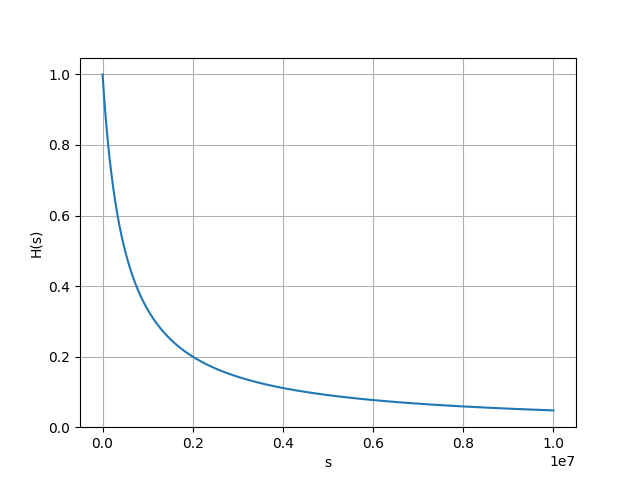
\includegraphics[width=\columnwidth]{figs/1_3.png}
    \caption{Plot of $H(s)$.}
    \label{fig:hs}
\end{figure}
Clearly, $H(s)$ is a low-pass filter.

\item Using trapezoidal rule for integration, formulate the difference
equation by considering 
\begin{align}
	y(n) = y(t)\vert_{t=n}
\end{align}

\solution Integrating \eqref{eq:diff-eqn} between limits $n-1$ to $n$ 
and applying the trapezoidal formula,
\begin{align}
    \frac{v_C\brak{n} + v_C\brak{n-1}}{2} + \tau\brak{v_C\brak{n}-v_C\brak{n-1}} \nonumber \\
    = \frac{V(n)+V(n-1)}{2}
    \label{eq:difference-eqn}
\end{align}
for $n > 0$, where $v(0) = 0$.
\item Find $H(z)$.

\solution Applying the Z-transform on both sides of \eqref{eq:difference-eqn},
\begin{align}
    V_C(z)\sbrak{(2\tau + 1) - z^{-1}(2\tau - 1)} = V(z)\brak{1 + z^{-1}}
\end{align}
Hence,
\begin{align}
    H(z) = \frac{1+z^{-1}}{\brak{2\tau+1}-\brak{2\tau-1}z^{-1}}
    \label{eq:Hz}
\end{align}
since $\abs{\frac{2\tau-1}{2\tau+1}} < 1$, the ROC is $\abs{z} > 1$.
\item How can you obtain $H(z)$ from $H(s)$?

\solution We use the bilinear transformation. Setting
\begin{align}
    s \triangleq \frac{2}{T}\frac{1 - z^{-1}}{1 + z^{-1}}
\end{align}
we get
\begin{align}
    H(z) = \frac{1}{1 + \frac{2\tau}{T}\frac{1-z^{-1}}{1+z^{-1}}}
\end{align}
Setting $T = 1$ gives \eqref{eq:Hz}.

\item Find $v_C(n)$. Verify using ngspice and the differential equation.

\solution Note that $v(n) = Vu(n)$. Thus,
\begin{align}
    V(z) = \frac{V}{1-z^{-1}}
\end{align}
Therefore,
\begin{align}
    V_C(z) &= H(z)V(z) \\
         &= \frac{TV\brak{1+z^{-1}}}{\brak{1-z^{-1}}\brak{\brak{2\tau+T}-\brak{2\tau-T}z^{-1}}} \\
         &= \frac{V\brak{1+z^{-1}}}{2}\sum_{k=-\infty}^{\infty}\brak{1-p^k}u(k)z^{-k}
\end{align}
where $p \triangleq \frac{2\tau-T}{2\tau+T}$. Thus,
\begin{align}
    &v_C(n) = \nonumber \\
    &\begin{cases}
        \frac{V}{2}\sbrak{u(n)\brak{1-p^n}+u(n-1)\brak{1-p^{n-1}}} & n > 0 \\
        0 & n \le 0
    \end{cases}
    \label{eq:vn}
\end{align}
We take $T = 10^{-7}$ as the
sampling interval. The python code \texttt{codes/1\_7.py} verifies
these equalities.
\begin{figure}
    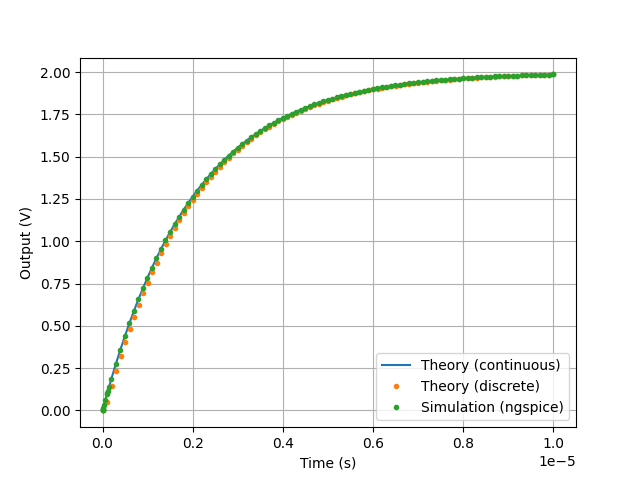
\includegraphics[width=\columnwidth]{figs/1_7.png}
    \caption{Representation of output across $C$.}
    \label{fig:vc}
\end{figure}
\end{enumerate}
\end{document}
